%results

                \begin{figure}[!ht]
		\begin{center}
		  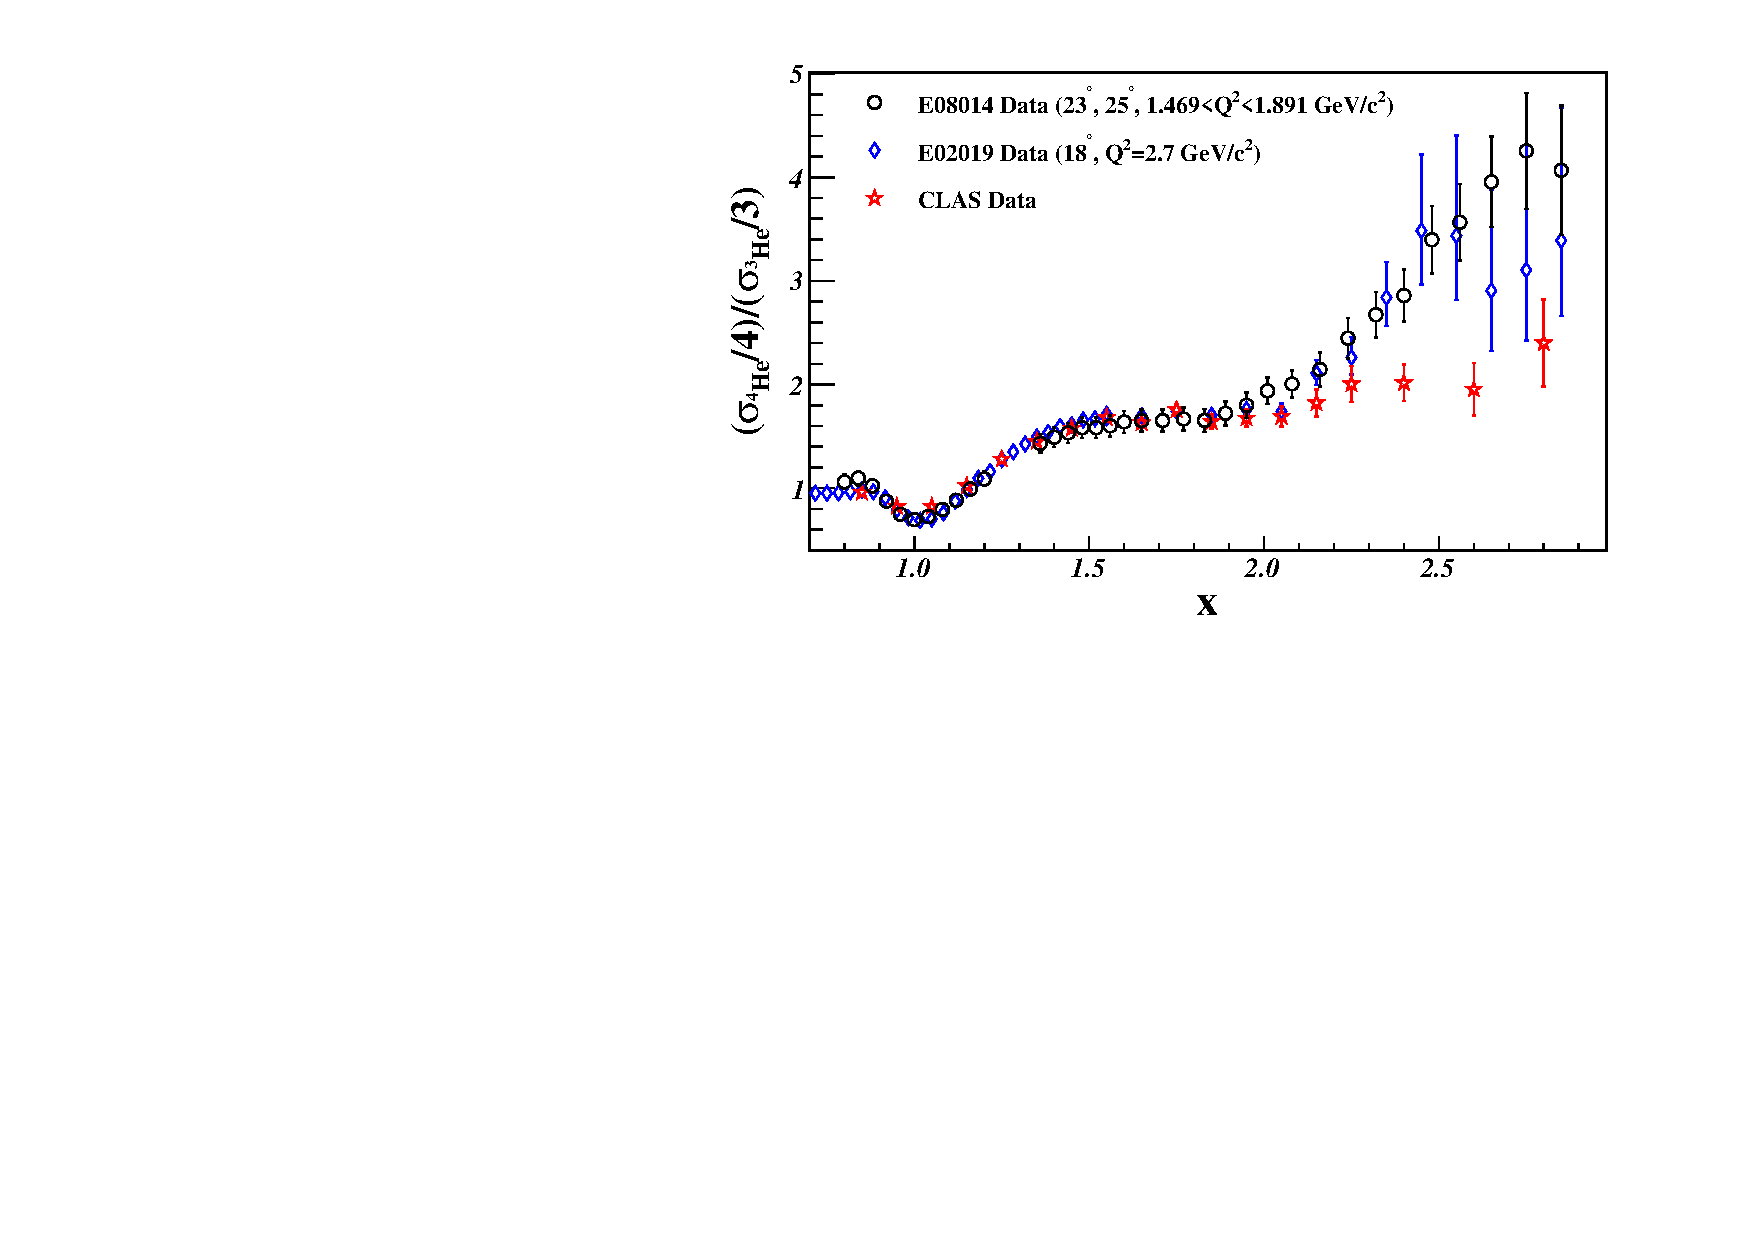
\includegraphics[width=8.5cm,angle=0]{He4_He3_XS_Ratio.pdf}
		\end{center}
		\vspace*{-5mm}
		\caption{(Color online) The $^4$He/$^3$He cross section ratio for $Q^2>1.4$~GeV$^2$ (23$^o$ and 25$^o$ scattering),
                  along with results from CLAS~\cite{PhysRevLett.96.082501} and Hall C (E02-019)~\cite{fomin2012}. The error bars include
                  statistical and systematic uncertainties; the global 5\% normalization uncertainty is not shown.}
		\label{fig:ratios_highqsq}
		\end{figure}

Figure~\ref{fig:ratios_highqsq} presents the $^4$He/$^3$He cross section ratio for our $Q^2 > 1.4$~GeV$^2$
data. In the 2N-SRC region, our data are in good agreement with the CLAS~\cite{PhysRevLett.96.082501} and
E02-019~\cite{fomin2012} results, revealing a plateau for $1.5 < x < 2$. At $x>2$, our
ratios are significantly larger than the CLAS data, but consistent within uncertainties with the E02-019
results. This is consistent with the explanation provided in a recent comment~\cite{Higinbotham:2014xna}
which concluded that the observed plateau was likely the result of large bin-migration effects resulting from
the limited CLAS momentum resolution.

While the rise in the ratio above $x=2$ indicates contributions beyond 2N-SRCs, we do not observe the 3N-SRC
plateau expected in the naive SRC model. In this model, the prediction of scaling as an indication of SRC
dominance is a simple and robust way to test for 2N-SRCs, but it is less clear how well it can indicate the
presence of 3N-SRCs. For 2N-SRCs, one can predict \textit{a priori} where the plateau should be observed
since for a given $Q^2$ value, $x$ can be chosen to require a minimum nucleon momentum above the Fermi
momentum, strongly suppressing single-particle contributions. It is not clear what values of $x$ and $Q^2$
are required to suppress 2N-SRC contributions well enough to isolate 3N-SRCs; much larger $Q^2$ values may
be required to isolate 3N-SRCs and see analogous plateaus at $x>2.5$.

                \begin{figure}[!ht]
		\begin{center}
		  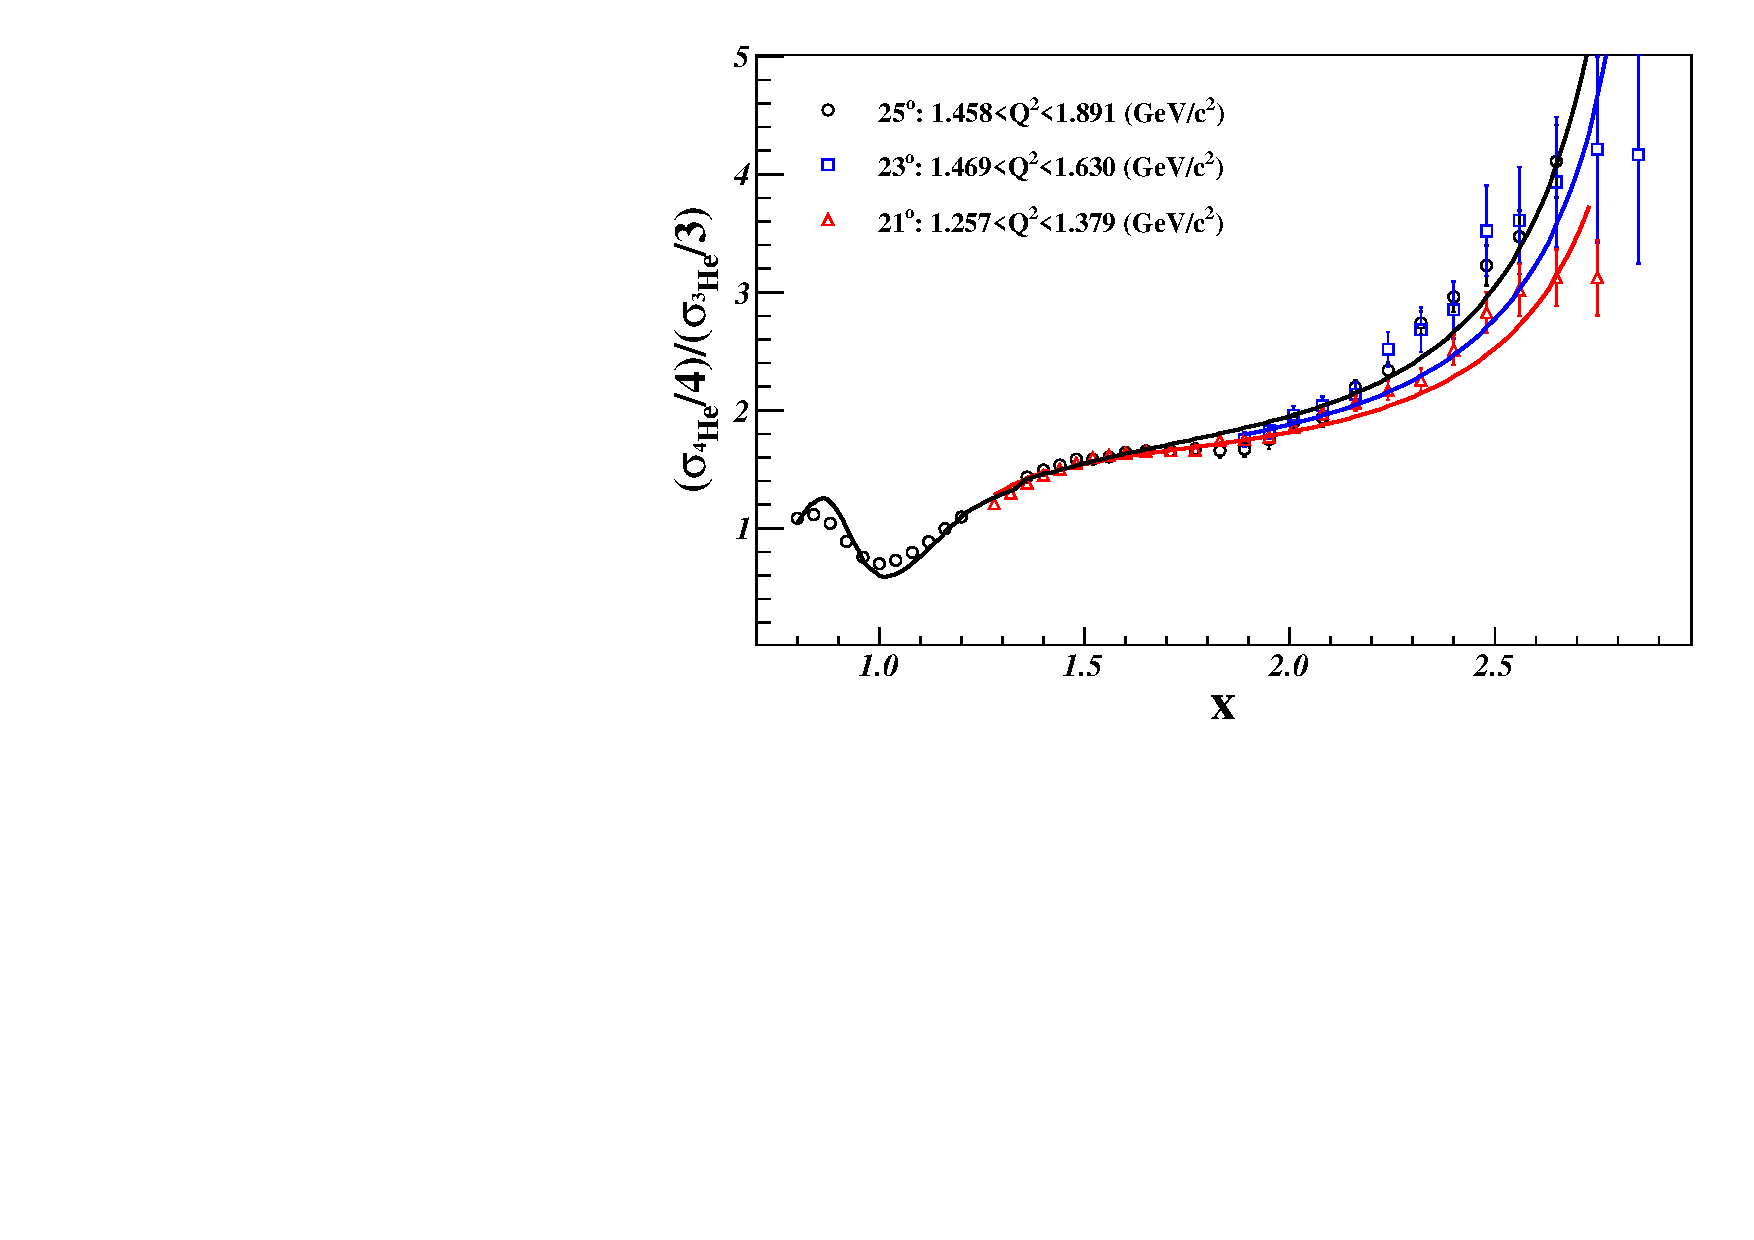
\includegraphics[width=8.5cm,angle=0]{He4_He3_XS_Ratio_MC}
                  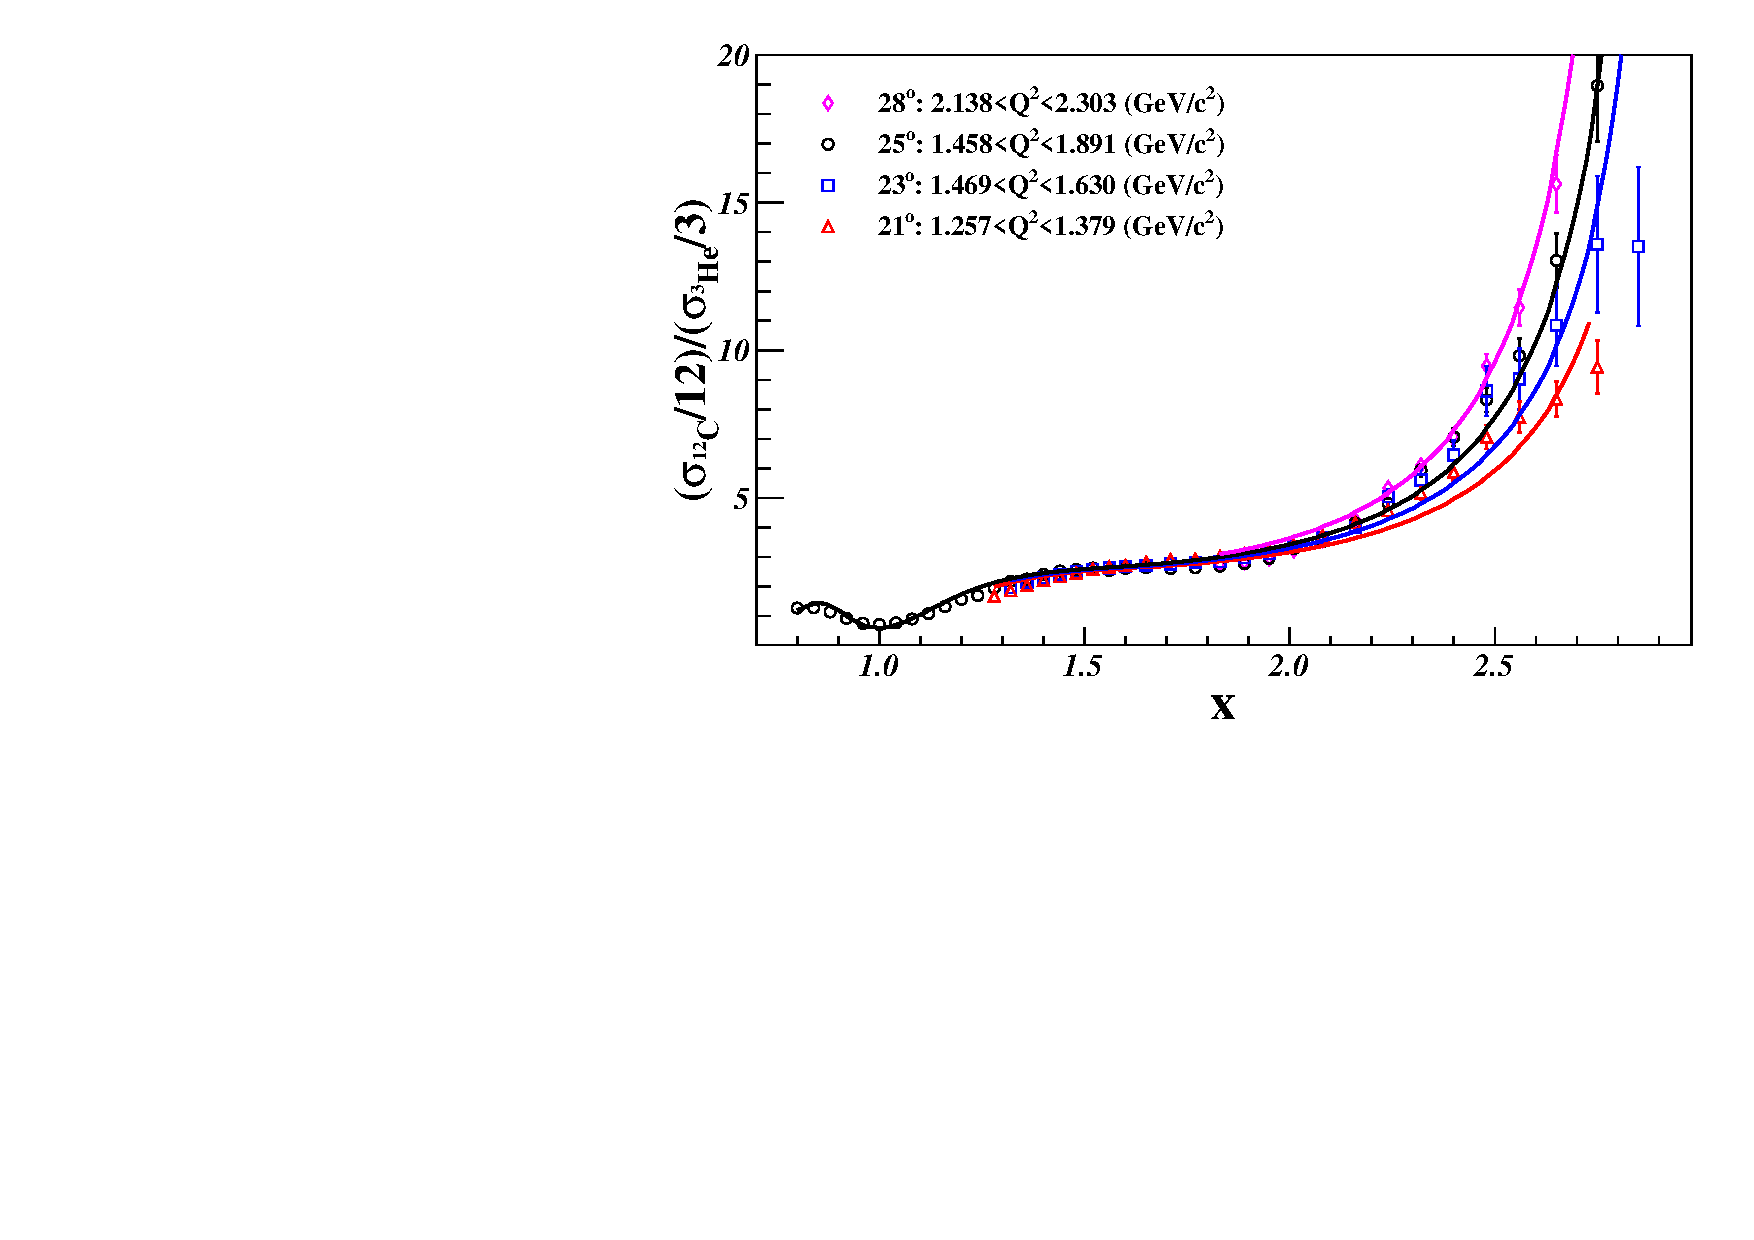
\includegraphics[width=8.5cm,angle=0]{C12_He3_XS_Ratio_MC}
		\end{center}
		\vspace*{-5mm}
		\caption{(Color online) The $^4$He/$^3$He (top) and $^{12}$C/$^3$He (bottom) cross section ratios for all angles, 
		  along with results from CLAS~\cite{PhysRevLett.96.082501} and Hall C (E02-019)~\cite{fomin2012} measurements. The solid lines
                  correspond to a simple cross section model based on parameterized momentum distributions.}
		\label{fig:ratios_allqsq}
		\end{figure}

For 2N-SRCs, the plateau must eventually disappear as the deuteron cross section falls to zero for $ x \to
M_D / M_p\approx 2$, causing the A/$^2$H ratio to rise sharply to infinity. Both the previous high-$Q^2$
deuterium data and our simple cross section model, based on a parameterization of the nulcon momentum
distribution in the nucleus, show that the
sharp drop of the deuteron cross section does not occur until $x \approx 1.9$, resulting in a clear plateau
for $1.5 < x < 1.9$. For $^3$He, our cross section model shows a similar falloff of the $^3$He cross section
starting near $x \approx 2.5$, thus yielding a rise in the A/$^3$He ratio that sets in at much lower $x$
values. This rapid rise in the A/$^3$He ratio as one approaches the $^3$He kinematic threshold shifts to
lower $x$ as $Q^2$ increases, as seen in both the data and model in Fig~\ref{fig:ratios_allqsq}. So while
the plateau is expected to set in at lower $x$ values as $Q^2$ increases, as seen in the 2N-SRC
region~\cite{ SLAC_Measurement_PRC.48.2451, PhysRevLett.96.082501}, the large-$x$ breakdown also shifts to
lower $x$ values. Thus, it is not clear whether higher $Q^2$ measurements will yield a clean way to isolate
and study 3N-SRCs.

                \begin{figure}[!ht]
		\begin{center}
		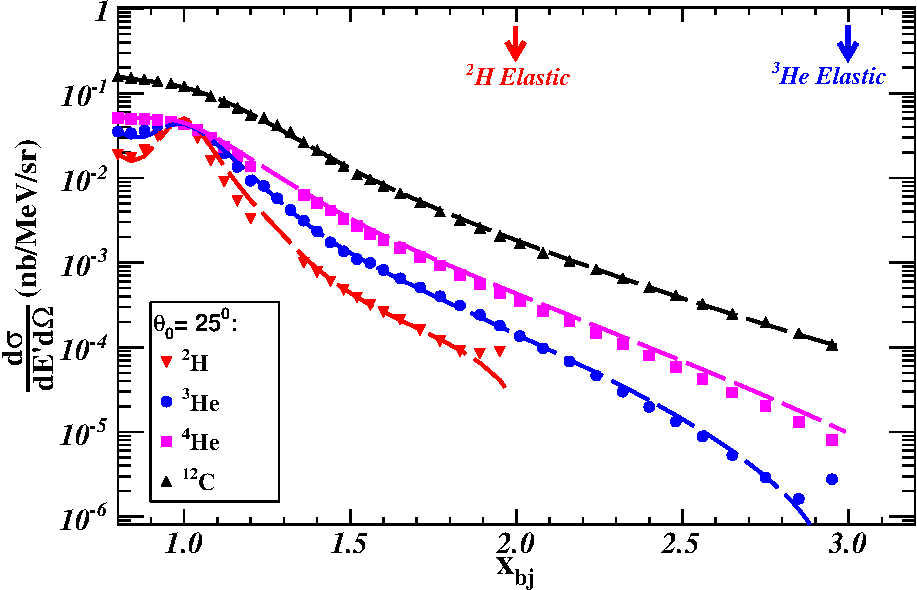
\includegraphics[width=8.5cm,angle=0]{Plot_XS_25_MC}
		\end{center}
		\vspace*{-5mm}
		\caption{(Color online) Cross sections of $^2$H, $^3$He, $^4$He and $^{12}$C at $25^{\circ}$. The uncertainties include statistical and
		systematic uncertainties. The normalization uncertainties, ranging from 2-5\%, are not shown.}
		\label{xs}
		\end{figure}

The absolute cross sections for scattering from $^{3}$He, $^{4}$He and $^{12}$C at a scattering angle of
$25^{\circ}$ are shown in Fig.~\ref{xs}. The $^3$He cross section falls more rapidly than the other nuclei
for $x>2.5$, yielding the rise in the $^4$He/$^3$He ratios discussed above. In the naive SRC model, it is
assumed that the high-$x$ cross section comes from the contributions of \textit{stationary} 2N- and 3N-SRCs.
The prediction of scaling in this model breaks down due to the difference between stationary SRC in $^2$H
(or $^3$He) and moving SRCs in heavier nuclei. For the most recent extraction of 2N-SRCs from the A/$^2$H
ratios~\cite{fomin2012}, the effect of the 2N-SRC motion in heavier nuclei was estimated and found to give a
small enhancement of the ratio in the plateau region, with little distortion of the shape until $x >
1.9$~\cite{fomin2012} where the ratio rises rapidly to infinity. For 3N-SRCs, motion of the correlations
produces a similar rise which begins well before the kinematic limit at $x \approx 3$. This picture is also
consistent with the observation that the $x > 2.5$ increase in the ratio is larger for $^{12}$C/$^3$He.
However, a clear interpretation of the large $x$ behavior of $^{12}$C/$^3$He is more difficult. At very large
$x$ values, where the cross section drops rapidly, the data are very sensitive to the spectrometer resolution.
When comparing two thin targets, or two extended targets, the acceptance and resolution effects cancel, 
stronly suppressing such effects in the target ratios. However, in the ratio of $^{12}$C/$^3$He, the variation
of the resolution with target length and the possible impact of correlations between the scattering angles and
the reconstructed target position can yield different resolution effects for the two targets. So while the
rise in the $^{12}$C/$^3$He can be explained by the comparison of moving 3N-SRCs to stationary ones, there
can be additional effects due to the difference in resolution between the foil targets and the 20cm ${3,4}$He
targets.


%\textit{impact of isospin dependence?}.


%In attempting to isolate 3N-SRC contributions, the situation is less straightforward. Both 2N and 3N SRCs yield contributions to the high-momentum
%tail. The fact that we do not see significant deviations from the 2N-SRC picture for $1.5<x<2$ suggests that the 3N-SRC contributions are generally
%much smaller. Unlike the case for 2N-SRCs, where $k>k_F$ suppresses single particle strength, there is not a clear way to define a threshold in $x$
%that will sufficiently suppress 2N contributions.  Approaching the kinematic limit at $x \approx 3$, the $^3$He cross section falls to zero and the
%ratio must go to infinity. However, while this occurs in a vary narrow $x$ window for the A/$^2$H ratios, the rise occurs over a larger range in $x$
%in this case.

%Thus, it is not clear that there will be a significant window in $x$ where one would expect to see a plateau, especially at the relatively modest
%$Q^2$ values measured here. In the present experiment, we observe a small but noticeable $Q^2$ dependence, in particular for $x \gtorder 2.5$. This
%is also observed in our simple $y$-scaling cross section model, and does not occur in the $^{12}$C/$^3$He ratio, indicating that it is the $x$
%dependence of the falloff of the $^3$He cross section as $x \to 3$ that is varying strongly with $Q^2$. Larger $Q^2$ values may be required to
%observe a $Q^2$-independent behavior of the ratios with $x$, which may allow us to isolate 3N-SRC contributions.



%\textit{Figure with A/2H ratios up to $x=2$, table with $a_2$ results for $A=3$, 4, 12, 48?}


%JRA Notes:
%0) Can we look at A/D ratios vs. Q^2 for our cross section model? Impact of x-->2 in 2H? Where does A/D rise up for x-->2?
%1) x-->3 has may have larger missing energy (plus, smaller energy step from x=1 to 2 to 3, so may fall to zero over wider range.
%2) $Q^2$ dependence of $x \to 3$ ratios in general agreement with what we observe in our cross section model. Suggests that the cross
%section falloff as we approach the kinematic threshold is large
